\begin{figure}[htbp]
\centering
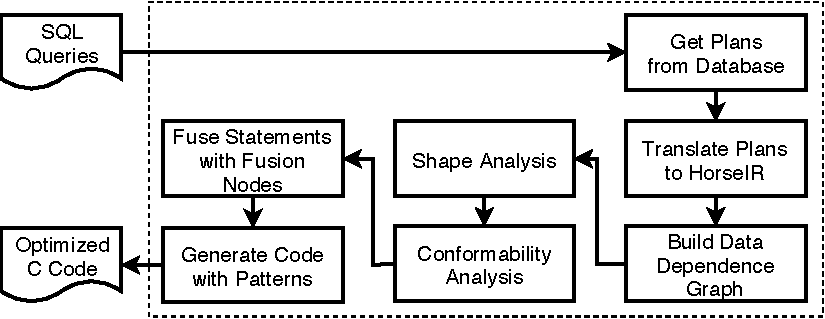
\includegraphics[width=\columnwidth]{./src/figure/overview-v4.pdf}
\caption{Analysis and code generation overview.} \label{fig:overview}
\end{figure}

We have implemented our approach for generating fused and efficient
\texttt{C} code in the HorseIR compiler. An overview of the workflow
can be found in \refFig{fig:overview}.

Just as in previous work~\OldPaper, we first generate an optimized
query execution plan using the HyPer database system~\cite{Neumann2011:HyPer}
from the input query, and translate this plan into HorseIR. 

Next, local data-flow analysis processes the intermediate program and
computes the shape information at each expression. Shapes are propagated
according to rules defined for each built-in function. Using the
generated shape information, we then employ conformability analysis to
identify fusible sections of code on a data-dependence graph.

Lastly, we optimize the set of fused sections using predefined patterns
and generate target C code. Patterns exploit additional optimization
opportunities that are frequently present in SQL queries.
